\section{热膨胀与温度测量}
\subsection{从温度变化到长度变化}
温度是描述物体热状态的量。两个物体接触后不再发生净热传递，称为达到热平衡；热平衡时温度相同。物体含有多少内能，还与物质的种类和多少有关，不能用内能大小定义温度。热量则是在温差作用下传递的能量，不是物体“含有”的状态量。

摄氏温度与热力学温度的换算写为
\[\frac T{\mathrm K}=\frac t{{}^\circ\mathrm C}+273.15.\]
温差的数值以K或摄氏度差表示相同，但温度之比必须用K。例如气态方程中的 $T$ 不能替换为摄氏温度；在热膨胀公式中，若只出现 $\Delta T$，则两种温差单位的数值可直接对应。部分题为计算方便取 $273$，应遵从该题约定，不能在同一计算中混用。


温度升高时，固体微观粒子的平均间距通常增大，宏观长度随之改变。在一段温区内，实验发现长度变化近似正比于原长与温差：

\[\Delta L=\alpha L_0\Delta T,\qquad L=L_0(1+\alpha\Delta T).\]
其中 $L_0$ 是基准温度 $T_0$ 下的长度，$\alpha$ 的单位是 $\mathrm{K^{-1}}$。此公式含两个近似：材料可自由膨胀，且该温区内 $\alpha$ 变化不明显。若杆被刚性支架固定，长度未必按上式实际增加，而可能产生热应力，此时还须结合弹性关系求解。

\fig{fv:h1:expansion}{自由杆的原长与伸长分开标记；图中伸长夸张绘制}{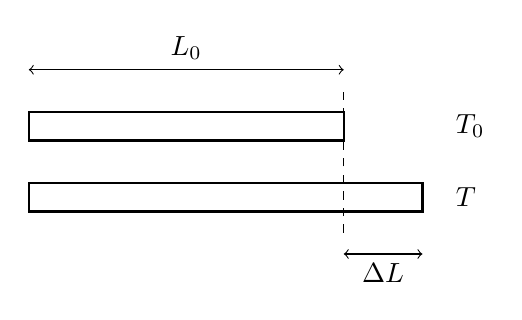
\begin{tikzpicture}[x=1cm,y=.9cm]
\draw[thick](0,1)rectangle(4,1.4);\draw[thick](0,0)rectangle(5,.4);\draw[dashed](4,-.3)--(4,1.7);
\draw[<->](0,2)--(4,2)node[midway,above]{$L_0$};\draw[<->](4,-.6)--(5,-.6)node[midway,below]{$\Delta L$};
\node[right]at(5.3,1.2){$T_0$};\node[right]at(5.3,.2){$T$};\end{tikzpicture}}
图\ref{fv:h1:expansion}中两次长度共用同一左端基准，虚线保留原右端的位置，向右多出的一段才是$\Delta L$。相对伸长应除以原长$L_0$；不能将升温后的$L$误作基准长度。若两端都受固定限制，图示自由伸长便不能实际发生，应另列约束和弹性关系。


从相对变化看，$\Delta L/L_0=\alpha\Delta T$。多数金属的 $\alpha$ 很小，所以在常见温差下可以保留一阶小量。若长度的变化进入周期、密度等非线性表达式，应先写精确的量之间关系，再统一展开，避免对不同量随意作同一种近似。

热膨胀系数给出的是材料的响应，题目要求的往往是装置的响应。以摆钟为例，温度先改变摆长，摆长再改变一次摆动所需的时间，最后才改变一天内完成的摆动次数。这三个环节应分别列式。若把“长度增加万分之几”直接当成“钟少走万分之几”，便忽略了周期对长度的平方根依赖。

对于随长度的幂次变化的量$Y\propto L^q$，令$\varepsilon=\alpha\Delta T$，先写$Y/Y_0=(1+\varepsilon)^q$。对$F(\varepsilon)=(1+\varepsilon)^q$求导，
\[
F'(\varepsilon)=q(1+\varepsilon)^{q-1},\qquad
F(0)=1,\quad F'(0)=q.
\]
在$|\varepsilon|\ll1$时，一阶展开$F(\varepsilon)=F(0)+F'(0)\varepsilon+O(\varepsilon^2)$才给出$\Delta Y/Y_0\simeq q\alpha\Delta T$。比较实际时间与仪器读数时，还须由计数方式判断应用的是周期本身，还是周期的倒数。

若膨胀系数显著依赖温度，可用微分定义 $\alpha=(1/L)(\dd L/\dd T)$。将变量分离为$\dd L/L=\alpha(T)\dd T$，并把基准状态$L(T_0)=L_0$作为积分下限，得到
\[
\int_{L_0}^{L}\frac{\dd\ell}{\ell}
=\int_{T_0}^{T}\alpha(\vartheta)\,\dd\vartheta,
\qquad
[\ln\ell]_{L_0}^{L}=\ln\frac{L}{L_0}.
\]
对两边取指数，才有$L/L_0=\exp[\int_{T_0}^{T}\alpha(\vartheta)\dd\vartheta]$。常系数时右侧积分为$\alpha(T-T_0)$，再展开$e^{\alpha\Delta T}=1+\alpha\Delta T+O((\alpha\Delta T)^2)$，便得到本讲使用的一阶模型。




\subsection{面积、体积、孔洞与复合结构}
对各向同性材料，三个方向按同一长度比例变化。因此面积与体积分别满足
\[\frac A{A_0}=(1+\alpha\Delta T)^2\simeq1+2\alpha\Delta T,\qquad
\frac V{V_0}=(1+\alpha\Delta T)^3\simeq1+3\alpha\Delta T.\]
令$\varepsilon=\alpha\Delta T$，平方与立方的实际展开为$1+2\varepsilon+\varepsilon^2$和$1+3\varepsilon+3\varepsilon^2+\varepsilon^3$。舍去二阶及更高项，才得到面积膨胀系数约为$2\alpha$、体膨胀系数约为$3\alpha$；前提是材料各向同性。质量不变时，先用$\rho V=\rho_0V_0$得$\rho/\rho_0=(1+\varepsilon)^{-3}$，再在上面的幂函数展开中取$q=-3$，得到$\rho\simeq\rho_0(1-3\alpha\Delta T)$。

孔洞随整体的几何尺度扩大。可把孔暂时用同种材料填满，整体自由、均匀膨胀后再取出填充部分；孔的边界会移动到相同的放大位置。这个论证要求自由膨胀，不能直接用于外边界被夹紧的金属环。

也可以从坐标来理解孔洞膨胀。若以任意一点为原点，自由均匀膨胀使每个材料点的坐标都乘 $1+\alpha\Delta T$。孔边界上的点服从相同的位移规律，因此孔半径也乘这一因子。它说明“孔变大”是整个位移场的结果，与孔内有没有填充物无关。若外缘受固定约束，位移场已经改变，便需要重新求解，不能仍沿用自由膨胀的结论。

\fig{fig:h1:holeconstraint}{自由圆环的内外边界按同一比例放大；两端固定的杆则建立压应力}{\begin{tikzpicture}

\draw[guide](0,0)circle(.8) (0,0)circle(1.6);\draw[blue,thick](0,0)circle(.92) (0,0)circle(1.84);\fill(0,0)circle(.04)node[below left]{$O$};\draw[flow](1.6,0)--(1.84,0);\draw[flow](0,.8)--(0,.92);\node at(0,-2.4){$a'=(1+\alpha\Delta T)a$};
\begin{scope}[xshift=7cm]\draw[world](0,-.8)--(0,.8) (4,-.8)--(4,.8);\draw[world](0,-.2)rectangle(4,.2);\draw[force](0,0)--(1,0)node[above]{$F$};\draw[force](4,0)--(3,0)node[above]{$F$};\node at(2,1.2){两端固定};\node at(2,-1.4){$\varepsilon_{\rm total}=0$};\end{scope}

\end{tikzpicture}}
图\ref{fig:h1:holeconstraint}左图中，材料点的位移沿半径向外，内边界并没有向孔内挤入。右图的杆却不能伸长：若再采用线弹性模型、杨氏模量为$E$，总应变由热应变与弹性应变相加，

\[
 0=\alpha\Delta T+\frac{\sigma_m}{E},\qquad
 \sigma_m=-E\alpha\Delta T.
\]
这里约定拉应力为正，故升温后的应力为压应力。这个结果来自固定端的几何限制；自由杆只有热伸长，不能同时再给它施加上述固定端应力。



复合杆、双金属结构和有间隙的装置应逐段写变化量，再列几何约束。串联自由杆的总长变化为 $\sum_i\alpha_iL_i\Delta T$；两个端点的间距变化则可能是两段伸长之差。解题时应在图上标出比较的两个端点，不能看到“加热”就把所有变化量相加。

若尺本身膨胀，每个刻度对应的实际长度也随之增加，读数应由“被测长度除以实际刻度长度”求出。尺与被测物同时升温时，一阶读数变化取决于两者膨胀系数之差，而不是只取其中一个系数。例\ref{t1-1}和练习\ref{t1-10}分别讨论时间测量与孔洞几何。

\section{表面张力与弯曲液面}
\subsection{表面张力的方向与两个表面的计数}
液体表层分子的环境不同于内部，形成液面需要能量。在给定温度和界面成分下，液面有减小面积的趋势。沿液面内任取一条边界线，邻侧液面对该线的作用力位于液面切平面内，方向垂直于该边界线。

对长度为 $\ell$ 的直边，一个液面贡献 $\sigma\ell$ 的拉力。肥皂膜由两面构成，若两面表面张力系数均为 $\sigma$，活动边受到的总拉力为 $2\sigma\ell$。这里的“两个表面”不能误解成边界线的左右各算一次；应直接数同一薄膜的正反两个气液界面。

\fig{fig:film-work}{双面膜活动边的受力与面积变化}{\begin{tikzpicture}[x=1cm,y=1cm]
\fill[blue!8] (0,0) rectangle (3,2);\draw[world] (0,2)--(0,0)--(3,0) (0,2)--(3,2);\draw[very thick] (3,0)--(3,2);\draw[guide] (4,0)--(4,2);\draw[force] (3,1)--(1.8,1) node[midway,above]{$2\sigma\ell$};\draw[force] (3,.45)--(4.3,.45)node[right]{$F_{\text{外}}$};\draw[flow] (3,2.5)--(4,2.5) node[midway,above]{$\dd x$};\draw[dim] (4.6,0)--(4.6,2) node[midway,right]{$\ell$};\begin{scope}[xshift=6cm]\draw[blue,thick](0,.5)--(1.5,.5) (0,.3)--(1.5,.3);\node at(.75,1.3){膜厚夸张的截面};\node[right]at(1.5,.8){正面};\node[right]at(1.5,0){反面};\end{scope}
\end{tikzpicture}}

图\ref{fig:film-work}的活动边向右移动 $\dd x$ 时，每面面积增加 $\ell\dd x$，总面积增加 $2\ell\dd x$。外力准静态做功 $2\sigma\ell\dd x$，恰等于表面自由能的增加 $\sigma\dd A_{\text{总}}$。因此 $\sigma$ 既可用 $\mathrm{N/m}$ 表示，也可用 $\mathrm{J/m^2}$ 表示；面积法与受力法是相互校验的两种方法。

恒温且 $\sigma$ 近似不变时，$\Delta F_{\text{表}}=\sigma\Delta A_{\text{总}}$。若温度变化明显或界面成分变化，$\sigma$ 也会变化，不能直接把全部表面能变化写成同一常数乘面积差。

\subsection{由局部受力确定曲率与压差}
受均匀膜张力作用的轻细线，平衡时曲率与张力有关。在光滑圆弧上取长度 $\dd s=r\dd\varphi$ 的微元，线两端张力的法向合力为 $\tau\dd\varphi$；双面膜的横向拉力为 $2\sigma\dd s$。因此

\[\frac\tau r=2\sigma.\]
\fig{fig:h1:lineelement}{弧形细线微元的两端张力合力向曲率中心，膜力沿法向向外}{\begin{tikzpicture}

\coordinate(A)at(1.691447,-.615636);\coordinate(B)at(1.691447,.615636);\draw[blue,very thick](A)arc(-20:20:1.8);\draw[guide](0,0)--(A) (0,0)--(B);\fill(0,0)circle(.04)node[left]{$O$};\node[below]at(.9,-.33){$r$};\draw(.6,-.218382)arc(-20:20:.638507);\node at(.95,0){$\dd\varphi$};
\draw[force](A)--(1.281023,-1.743267)node[below]{$\tau$};\draw[force](B)--(1.281023,1.743267)node[above]{$\tau$};\draw[force](1.8,0)--(3.2,0)node[right]{$2\sigma\dd s$};\node[right]at(1.9,.65){$\dd s=r\dd\varphi$};

\end{tikzpicture}}
图\ref{fig:h1:lineelement}把“沿细线的张力$\tau$”与“膜对细线的分布拉力$2\sigma$”分开。前者在两端分别沿切线，后者垂直线元；两端张力的方向差才提供$\tau\dd\varphi$，不能把两个张力大小直接相加为$2\tau$。



上述微元平衡还说明自由段为什么是圆弧。轻线处处无切向分布力，张力的大小沿线不变；膜的单位长度拉力也是常量，所以 $1/r=2\sigma/\tau$ 处处相同。曲率恒定的平面曲线就是圆弧。应先确定这条局部关系，再用全局长度和容许区域确定圆弧的位置。若所需圆弧越过容器边界，继续增加的线长只能通过接触段等方式容纳。

局部关系只决定弯曲段的半径，还必须满足端点、长度和边界接触条件。例\ref{t1-2}中长线不能全部画成自由优弧，应检查上下边界是否阻止圆弧继续延伸。

球形液面也可由整体受力求附加压强。图\ref{fig:laplace}取上半球，向上的压差合力作用在圆形截面，沿边缘向下的表面张力作用于整个圆周。取半球，截面上的压差合力是 $\Delta p\,\pi r^2$，圆周表面张力合力是 $2\pi r\sigma$，所以

\[\boxed{\Delta p=\frac{2\sigma}{r}}.\]
对液滴或液体中的单界面气泡，内侧压强均比紧邻外侧高 $2\sigma/r$；薄肥皂泡有两个表面，近似为 $\Delta p=4\sigma/r$。判断压差符号时，应先画出表面张力对半球的作用方向，再列平衡方程。不能单凭“里面是气体还是液体”决定压差正负。

\fig{fig:laplace}{半球截面上的压差合力，与截面圆周上的表面张力相平衡}{\begin{tikzpicture}

\fill[blue!8](0,0)arc(180:0:1.2)--cycle;\draw[world](0,0)arc(180:0:1.2);\draw[guide](0,0)--(2.4,0);\draw[force](1.2,.2)--(1.2,2)node[above]{$(p_{\rm in}-p_{\rm out})\pi r^2$};\draw[force](0,0)--(0,-.9);\draw[force](2.4,0)--(2.4,-.9);\node at(1.2,-1.35){圆周总拉力$2\pi r\sigma$};\draw[dim](1.2,-.4)--(2.4,-.4)node[midway,below]{$r$};

\end{tikzpicture}}

\subsection{润湿、接触角与毛细高度}
液体与固体接触时，界面形状取决于几种界面的相互作用。接触角 $\theta$ 在液体一侧量取：$\theta<90^\circ$ 为润湿，弯月面通常凹向气体；$\theta>90^\circ$ 为不润湿，弯月面通常凸向气体。画接触角时，必须使用液面的切线，不能用连接两端的水平弦代替切线。

取半径 $r$ 的润湿毛细管中高于槽面的液柱，如图\ref{fig:h1:capillarybalance}左侧；右侧将这段液柱的剩余竖直作用单独画出。接触线总长 $2\pi r$，表面张力的竖直合力为 $2\pi r\sigma\cos\theta$。忽略弯月面体积，液柱重力为 $\rho g\pi r^2h$，故

\[\boxed{h=\frac{2\sigma\cos\theta}{\rho gr}}.\]
\fig{fig:h1:capillarybalance}{润湿液柱的高度与等效竖直受力；左图以$\theta=60^\circ$示意}{\begin{tikzpicture}

\draw[world](0,-.5)--(0,2.8) (.8,-.5)--(.8,2.8);\draw[guide](-.8,0)--(2,0)node[right]{槽面};\fill[blue!8](0,0)--(0,1.7)arc(240:300:.8)--(.8,0)--cycle;\draw[blue,thick](0,1.7)arc(240:300:.8);
\draw[guide](0,1.7)--(.6,1.35359);\draw(0,1.4)arc(-90:-30:.3);\node[right]at(.18,1.2){$\theta$};\draw[dim](1.5,0)--(1.5,1.6)node[midway,right]{$h$};\draw[force](0,1.7)--(-.8,2.16188);\draw[force](.8,1.7)--(1.6,2.16188);
\begin{scope}[xshift=5.5cm,yshift=.8cm]\fill(0,0)circle(.07);\draw[force](0,0)--(0,1.4)node[above]{$2\pi r\sigma\cos\theta$};\draw[force](0,0)--(0,-1.4)node[below]{$\rho g\pi r^2h$};\end{scope}

\end{tikzpicture}}
图\ref{fig:h1:capillarybalance}左图接触线处的箭头沿界面切线，两个箭头是整个圆周拉力的截面示意。以方位角$\varphi$参数化接触圆周，$\dd\ell=r\dd\varphi$；每段竖直拉力为$\sigma\cos\theta\,\dd\ell$，所以
\[
F_z=\int_0^{2\pi}\sigma r\cos\theta\,\dd\varphi
=\sigma r\cos\theta[\varphi]_0^{2\pi}
=2\pi r\sigma\cos\theta.
\]
这才是右图所标的总力。忽略弯月面体积时，液柱体积近似为$\pi r^2h$，所以周长与面积不同的尺度依赖给出$h\propto1/r$。



$h$ 是带符号的液面相对高度，润湿时为正，不润湿时为负。由公式可见管越细、毛细效应越显著；这来自张力随周长变化、重力随面积变化，而不是细管“吸力更强”的额外机制。

毛细高度也可由压强验证。润湿液面的曲率半径约为 $r/\cos\theta$，气体一侧压强比液面下方高 $2\sigma\cos\theta/r$。从槽面沿液体向上走 $h$，液体压强降低 $\rho gh$，两种压差相等，仍得到同一高度。受力法取的是整段液柱，压强法比较的是液面两侧；把两种方法的力或压差重复相加，会把同一表面作用算两次。

上述推导假设槽面近似不动、管径远小于毛细高度，且液面已达到平衡。若两管连接有限容积液槽，应再列液体体积守恒。若存在快速流动，黏性阻力与动态接触角也会影响过程，静态毛细高度不能代替流量公式。

植物输水中，毛细作用可以说明局部弯月面压差，但完整运输还涉及蒸腾引起的水势差及连续水柱等条件。将静态毛细高度直接当作植物输水的全部解释，会混淆局部平衡与持续输运。

\fig{fig:contact-angle-sign}{接触角从液体一侧量取，界面切线决定张力竖直分量；弯月面作局部示意}{
\begin{tikzpicture}[x=1.1cm,y=1.1cm]
\foreach \s in {0,4.4}{\begin{scope}[xshift=\s cm]
\draw[world] (0,-1.5)--(0,1.5) (.8,-1.5)--(.8,1.5);
\draw[guide] (-.8,0)--(1.7,0);\node[right] at (1.7,0){槽面};
\end{scope}}
\fill[blue!10] (0,-1.5)--(0,.8) .. controls (.2,.6) and (.6,.6) .. (.8,.8)--(.8,-1.5)--cycle;
\draw[world] (0,.8) .. controls (.2,.6) and (.6,.6) .. (.8,.8);
\draw[guide] (0,.8)--(.48,.32);\draw[force] (0,.8)--(-.55,1.35);\draw[force] (.8,.8)--(1.35,1.35);
\draw (0,.56) arc(-90:-45:.24);\node at (.23,.48){$\theta$};
\node[align=center] at (.4,-2){$\theta<90^\circ$\\$\cos\theta>0,\ h>0$};
\begin{scope}[xshift=4.4cm]
\fill[blue!10] (0,-1.5)--(0,-.8) .. controls (.2,-.6) and (.6,-.6) .. (.8,-.8)--(.8,-1.5)--cycle;
\draw[world] (0,-.8) .. controls (.2,-.6) and (.6,-.6) .. (.8,-.8);
\draw[guide] (0,-.8)--(.48,-.32);\draw[force] (0,-.8)--(-.5,-1.3);\draw[force] (.8,-.8)--(1.3,-1.3);
\draw (0,-1.04) arc(-90:45:.24);\node at (.32,-.99){$\theta$};
\node[align=center] at (.4,-2){$\theta>90^\circ$\\$\cos\theta<0,\ h<0$};
\end{scope}
\end{tikzpicture}}
图\ref{fig:contact-angle-sign}中，箭头表示接触线处作用于液体的张力方向，沿气液界面的切线指向边界。润湿时其竖直分量向上，不润湿时向下；改变的不是 $\sigma$ 的正负，而是 $\cos\theta$ 的正负。对不润湿的下降液面，宜用压强法统一处理：
\[
 p_0-p_{\text{液面下}}=\frac{2\sigma\cos\theta}{r},
 \qquad p_0-p_{\text{液面下}}=\rho gh.
\]
两式都按同一方向取压差，因而给出同一个带符号高度公式。此时不能把“槽面以上的一段液柱”当作实际存在的正高度液柱，再给其重力随意加负号。图中的槽面是固定参考高度，$h<0$ 表示管内液面低于它。

\section{理想气体与液柱压强}
\subsection{状态量、绝对压强与理想气体近似}
描述定量平衡气体通常使用压强 $p$、体积 $V$ 和绝对温度 $T$。压强是气体对边界单位面积的法向作用，体积是气体实际占据的空间，温度反映热运动状态。理想气体模型忽略分子自身占有的体积及分子间势能；气体稀薄且远离凝结时，通常较为适用。

理想气体状态方程为
\begin{equation}\label{eq:t1state}
pV=nRT=NkT,\qquad n=\frac m\mu,\quad N=nN_A,\quad k=\frac R{N_A}.
\end{equation}
其中 $n$ 是物质的量，$N$ 是分子数，$\mu$ 是摩尔质量，三者不能混写。使用SI单位时 $p$ 用Pa，$V$ 用 $\mathrm{m^3}$，$\mu$ 用kg/mol，$R=8.314\,\mathrm{J/(mol\,K)}$。

式\eqref{eq:t1state}中的 $p$ 是相对于真空的绝对压强。若压力计给的是表压 $p_g$，应换成 $p=p_0+p_g$；只有在求活塞净受力时，才可直接用两侧压差乘面积。常见的错误是把表压代入气态方程，却在另一状态使用绝对压强。


固定气体量时，状态方程给出三种基本过程：等温 $pV=\text{常量}$，等容 $p/T=\text{常量}$，等压 $V/T=\text{常量}$。每一种关系都还包含“气体量固定”这一条件，漏气、充气、凝结或化学反应时必须重新检查。

在 $p$--$V$ 图上，等温线是双曲线，等容线竖直、等压线水平。在 $p$--$T$ 图上，等容线是过原点的射线，斜率 $nR/V$；在 $V$--$T$ 图上，等压线是过原点的射线，斜率 $nR/p$。若横轴采用摄氏温度，直线一般不再过坐标原点。

\fig{fig:h1:stateplots}{固定气体量时的过程图；温度坐标必须使用热力学温度}{\begin{tikzpicture}

\draw[axis](0,0)--(3.7,0)node[right]{$V$};\draw[axis](0,0)--(0,3.2)node[above]{$p$};\draw[blue,thick,domain=.8:3.3,samples=80]plot(\x,{2/\x});\draw[red,thick](.6,1)--(3.3,1);\draw[green!50!black,thick](2,.4)--(2,2.8);\fill(2,1)circle(.05);\node[blue]at(3,2.2){等温};\node[red]at(3,1.35){等压};\node[green!50!black]at(1.8,3.2){等容};
\begin{scope}[xshift=5.3cm]\draw[axis](0,0)--(3.6,0)node[right]{$T$};\draw[axis](0,0)--(0,3.2)node[above]{$p$};\draw[blue,thick](0,0)--(3.1,2.3);\node at(1.8,3.1){$V$固定};\node at(1.7,-1){斜率$nR/V$};\end{scope}
\begin{scope}[xshift=10.5cm]\draw[axis](0,0)--(3.6,0)node[right]{$T$};\draw[axis](0,0)--(0,3.2)node[above]{$V$};\draw[red,thick](0,0)--(3.1,2.3);\node at(1.8,3.1){$p$固定};\node at(1.7,-1){斜率$nR/p$};\end{scope}

\end{tikzpicture}}
图\ref{fig:h1:stateplots}左图三种过程可经过同一状态，但它们的后续路径不同。中图、右图的直线通过$T=0$的坐标原点是理想气体关系的数学外推；实际气体在极低温可能凝结，不能据外推断定模型在那里仍适用。用摄氏温度作横坐标时，只平移横轴，不能仍强令直线经过新原点。



两个平衡态之间总可写 $p_1V_1/T_1=p_2V_2/T_2$，但这只是端点关系，不能据此断定中间全过程等压、等温或等容。例\ref{t1-5}中三个阶段共用同一端点状态方程，却分别由不同机械约束确定路径。

\subsection{液柱压强与多液面联动}
静止液体中，取底面积$S$、高度$\dd z$的竖直薄层，向上为正。底面压力、顶面压力与重力平衡给出$p(z)S-p(z+\dd z)S-\rho gS\dd z=0$，除以$S\dd z$并取极限得$\dd p/\dd z=-\rho g$。若密度均匀，从$z_1$积分到$z_2$，
\[
\int_{p_1}^{p_2}\dd p=-\rho g\int_{z_1}^{z_2}\dd z,
\qquad p_2-p_1=-\rho g(z_2-z_1),
\]
故$p+\rho gz=\text{常量}$。沿同一连续液体向下走高度$h$，压强增加$\rho gh$；向上走则减小。同一水平面等压的结论只能用于同种、连通且静止的液体，不能跨过隔板或气体直接使用。

\fig{fig:hydrostatic}{同一液体内从开口端到气体端的压强传递}{\begin{tikzpicture}[x=1cm,y=1cm]
\draw[world] (0,3)--(0,0)--(3,0)--(3,2.5) (.4,3)--(.4,.4)--(2.6,.4)--(2.6,2.5);\draw[thick] (0,2.3)--(.4,2.3) (2.6,1.2)--(3,1.2);\draw[guide] (-.3,1.2)--(3.3,1.2);\node[above] at (.2,3){$p_0$};\node[above] at (2.8,2.5){$p$};\draw[dim] (3.8,1.2)--(3.8,2.3) node[midway,right]{$\Delta h$};\node at (1.6,-.7){$p=p_0+\rho g\Delta h$};
\end{tikzpicture}}

图\ref{fig:hydrostatic}中先从左液面向下到辅助水平面，再沿该水平面走到右液面，得到 $p=p_0+\rho g\Delta h$。若气体侧液面更高，$\Delta h$ 应取负。建议始终保留高度坐标，最后再代入数值，避免凭记忆写出错误的正负号。

液面发生位移时，还要满足液体体积守恒。若一U管两臂截面为 $S_1,S_2$，带符号液面位移满足 $S_1\delta h_1+S_2\delta h_2=0$。等截面才有两侧位移大小相等；由此得到的液面高度差变化常为单侧位移的两倍。例\ref{t1-3}用两组体积守恒再联系同一封闭气体，例\ref{t1-4}还须把管顶固定转化为空气柱长度变化。


理想混合气体中，每种组分可用其物质的量定义分压：$p_iV=n_iRT$，总压 $p=\sum_i p_i$。分压对应同一最终体积与温度，不能把不同容器、不同温度的初压直接相加。

若多个刚性容器等温连通且连通管体积可忽略，气体总量守恒，得到 $p_f\sum V_i=\sum p_iV_i$。若初温不同，应先列总内能守恒或与环境的能量交换，求出末温后再用状态方程。饱和蒸气还可能凝结或汽化，气相物质的量未必固定，这将在第四讲单独处理。

\section{活塞、轻绳与分段过程}
\subsection{机械平衡怎样确定气体路径}
状态方程只能联系 $p,V,T$，还需要机械条件确定过程。轻活塞在恒定外压下自由、缓慢运动时，两侧压强相等，因而气体可近似等压；重活塞竖直放置时，平衡压强为 $p=p_0+mg/S$；水平弹簧活塞则满足 $p=p_0+kx/S$，通常不是等压过程。

\fig{fig:piston-forces}{负载与挡板反力共同确定活塞压强；挡板反力只在接触时存在}{\begin{tikzpicture}

\foreach \j/\lab in {0/轻活塞,1/重活塞,2/重活塞接触上挡板}{\begin{scope}[xshift={4.6*\j*1cm}]
\draw[world](0,2.7)--(0,0)--(1.8,0)--(1.8,2.7);\fill[blue!8](0,0)rectangle(1.8,1.2);\draw[very thick](0,1.2)--(1.8,1.2);\node at(.9,.5){$p$};\node at(.9,2.4){$p_0$};\node at(.9,-.55){\lab};
\draw[force](.4,1.2)--(.4,2.1)node[left]{$pS$};\draw[force](1.4,2.1)--(1.4,1.2);\end{scope}}
\node at(1.8,1.8){$p_0S$};\node[align=left]at(6.9,1.7){$p_0S$\\$+mg$};\node[align=left]at(11.5,1.7){$p_0S$\\$+mg+N$};\draw[world](9.2,1.2)rectangle(11,1.35);\draw[world,very thick](9.2,1.35)--(11,1.35);
\node at(.9,-1.25){$p=p_0$};\node at(5.5,-1.25){$p=p_0+mg/S$};\node at(10.1,-1.25){$p=p_0+(mg+N)/S$};

\end{tikzpicture}}

图\ref{fig:piston-forces}显示同一气体方程对应不同机械路径。上挡板接触时，挡板可向下提供支持力，因此气体压强可超过自由平衡值而活塞仍不动。挡板撤去或支持力降为零，才切换到自由运动段。


轻绳只能拉，不能推；张力 $\tau\ge0$。计算得到负张力，通常表示“绳绷直”的假设失效，应改用绳松弛的约束。接触支持力同样只能指向阻止物体穿过边界的方向。若某段计算需要挡板把活塞拉回来，该段就不成立。

分段分析可按照以下顺序进行：先假定当前接触和绳状态；对每个活塞列受力平衡；用位置写气体体积；结合气态方程求状态变化；最后检查接触、张力和几何边界。某个不等式首次达到等号，便是下一段的起点。

在同一段中应消去不必要的未知量。例如两个活塞由绳连接且同时自由，分别列平衡后消去张力，往往可以先确定压强；再由绳长守恒把两个位移归结为一个坐标。台阶管中，两个活塞同向移动也可能使气体体积减小，体积应按各段截面积乘长度重新求和。

“接触挡板”与“自由运动”应由受力连续地衔接。例如重活塞靠在上挡板上时，$N=(p-p_0)S-mg\ge0$，压强可以高于自由平衡值。冷却使 $N$ 逐渐减小，只有减到零，活塞才开始离开；若继续把它当作固定边界，就会算出负的 $N$。反过来，自由运动段中位置达到挡板是几何临界条件，此刻支持力尚为零，随后升温才逐渐建立支持力。临界状态同时满足相邻两段的条件，因此可用它检查分段公式是否连续。

同理，对连接两活塞的绳，应先标清气体在哪一侧。气体对两活塞的压力未必同向，两个压差力也未必使用同一面积。先逐个活塞列式再消去张力，才能判断共同移动是等压过程还是变压过程。

例\ref{t1-8}训练“自由平移—接触台阶”的转换；例\ref{t1-9}包含“共同移动—固定体积—绳松弛”三段。解答不能只给一条折线，还要说明每个转折点对应装置中的哪个事件，临界张力与支持力是否符合方向约束。

\subsection{可逆绝热过程中的临界状态}
例\ref{t1-7}还需把受力确定的临界压强换算成温度。这里先使用定量理想气体的可逆绝热关系；其完整推导与自由膨胀的比较见热学第三讲。若热容恒定、过程缓慢无摩擦且无热交换，初态为 $(p_1,T_1)$、临界态为 $(p_2,T_2)$，则

\[
 \frac{T_2}{T_1}=\left(\frac{p_2}{p_1}\right)^{(\gamma-1)/\gamma},
 \qquad \gamma=\frac{C_p}{C_V}>1.
\]
先对气缸壳体列竖直受力平衡，令地面支持力首次降为零，求得 $p_2$；再将这个压强代入温度比。这样，离地条件由机械约束确定，达到该状态所需的温度由热学路径确定，两步各有独立作用。压缩时 $p_2>p_1$会给出 $T_2>T_1$，也可用来检查指数的正负。仅有“缸壁绝热”而过程不满足上述条件时，不能直接使用这个幂律。

